\documentclass[10pt,twocolumn]{article}

\usepackage[a4paper,margin=20mm,columnsep=7.5mm]{geometry}
\usepackage[T1]{fontenc}
\usepackage{lmodern}
\usepackage{microtype}
\usepackage{amsmath,amssymb,amsthm}
\usepackage{booktabs}
\usepackage{graphicx}
\usepackage{array}
\usepackage{enumitem}
\usepackage[dvipsnames]{xcolor}
\usepackage[numbers,sort&compress]{natbib}
\usepackage[colorlinks=true,allcolors=MidnightBlue]{hyperref}

\graphicspath{{figures/}{../results/decisive/}}
\setlength{\parindent}{1em}
\setlength{\parskip}{0pt}
\setlength{\tabcolsep}{4pt}
\renewcommand{\arraystretch}{1.12}
\linespread{1.03}
\raggedbottom

\newcommand{\MI}{\operatorname{I}}
\newcommand{\Var}{\operatorname{Var}}
\newcommand{\E}{\operatorname{E}}
\newcommand{\phat}{\widehat{P}}
\newcommand{\qhat}{\widehat{Q}}
\newcommand{\method}{Daniel's Method}
\newtheorem{proposition}{Proposition}

\title{\vspace{-1.2em}\textbf{Fast Differential Mutual Information Inference with a
Bias-Corrected Welch--Satterthwaite Reference}}
\author{\textbf{Daniel Zhao}\\
\small Master's Research in Information Theory\\
\small Draft methods article}
\date{\small 28 July 2026}

\begin{document}

\maketitle

\begin{abstract}
Mutual information (MI) quantifies arbitrary statistical dependence, yet
standard significance procedures are primarily designed to test independence
within one population. A different scientific question arises when two
independent populations may have distinct joint distributions but the same
strength of dependence: \(H_0:\MI(P)=\MI(Q)\), allowing \(P\ne Q\). Resampling
can address this weak null but is computationally costly, whereas a
bias-corrected influence-function Wald test is fast but can be liberal in
finite samples. We propose a deterministic refinement, termed \emph{\method},
that combines the classical first-order correction for discrete plug-in MI,
an empirical influence-function standard error, and a
Welch--Satterthwaite-inspired Student reference. The estimator, standard error,
and test statistic are unchanged from the normal Wald baseline; only the
reference distribution and confidence-interval critical value change.

The method was evaluated on 1.22 million weak-null table pairs and 50,000
power pairs spanning square and rectangular alphabets from \(2\times2\) to
\(20\times20\), balanced and skewed margins, and sample-size ratios up to
1:4. At nominal \(\alpha=0.05\), mean absolute false-positive-rate error fell
from 0.01177 to 0.01084 in the targeted hard grid, a 7.9\% relative
improvement, while broad-grid error changed from 0.00514 to 0.00504.
An independently generated holdout confirmed the direction of the effect.
Mean power loss was 0.00154, and median runtime was 0.128 ms versus 0.117 ms
for the normal test. Studentized permutation remained better calibrated
(hard-grid error 0.00642) but was substantially slower. An adversarial audit
showed that the implemented component degrees of freedom are heuristic for
plug-in influence variances, so the procedure is not an exact finite-sample
Welch test. The evidence supports a low-cost, mildly conservative refinement
for regular differential-MI inference, not a universal solution to sparse
tables or independence.
\end{abstract}

\noindent\textbf{Keywords:} mutual information; differential mutual
information; Welch--Satterthwaite approximation; influence function;
finite-sample inference; permutation test

\section{Introduction}

Mutual information (MI) is a model-free measure of statistical dependence
introduced by Shannon \citep{shannon1948}. For categorical variables it
summarizes the departure of a joint distribution from the product of its
margins and detects associations that need not be linear, monotone, or
low-dimensional. These properties make MI attractive in neuroscience,
genomics, ecology, remote sensing, and complex-systems research
\citep{brillinger2004,lizier2014}.

Most familiar MI significance procedures answer a one-population question:
are \(X\) and \(Y\) independent, or equivalently, is \(\MI(X;Y)=0\)?
The likelihood-ratio statistic \(2n\widehat{\MI}\) has an asymptotic
chi-squared reference for fixed categorical alphabets, and permutation
procedures commonly shuffle one variable to destroy dependence. Toolkits such
as JIDT make these calculations accessible \citep{lizier2014}.

Many comparative studies require a different test. Suppose the same
categorical variables are measured in two independent populations, such as
treatment and control, two environments, or two time periods. The question is
then
\begin{equation}
  H_0:\MI(P)=\MI(Q)
  \quad\text{against}\quad
  H_1:\MI(P)\ne\MI(Q),
  \label{eq:null}
\end{equation}
where the full joint distributions \(P\) and \(Q\) may differ. This is a
\emph{weak null}: equal MI does not imply equal margins, cell probabilities,
or association patterns. A chi-squared independence test in either table does
not answer Eq.~\eqref{eq:null}. Likewise, JIDT's standard shuffled
independence significance API is not a direct comparator.

The usual analytic route treats MI as a smooth multinomial functional away
from independence. A delta-method or influence-function calculation gives an
asymptotically normal estimator, and two independent variance contributions
can be added. For finite samples, however, the plug-in MI estimate is biased
upward and its estimated uncertainty is itself noisy. Unequal sample sizes
make the leading bias differ between groups. A normal-reference Wald test can
therefore reject too often in skewed or low-expected-count regimes.

This article studies a deliberately small modification. \method{} first
applies the classical \(O(n^{-1})\) bias correction to each MI estimate,
studentizes their difference using empirical local-information variances, and
then replaces the standard-normal reference by a Student distribution whose
effective degrees of freedom use the Welch--Satterthwaite formula
\citep{satterthwaite1946,welch1947}. The conceptual pipeline is shown in
Fig.~\ref{fig:pipeline}. Because every operation is computed directly from two
count tables, the method is deterministic and has \(O(rc)\) cost once the
tables are formed.

\begin{figure*}[t]
  \centering
  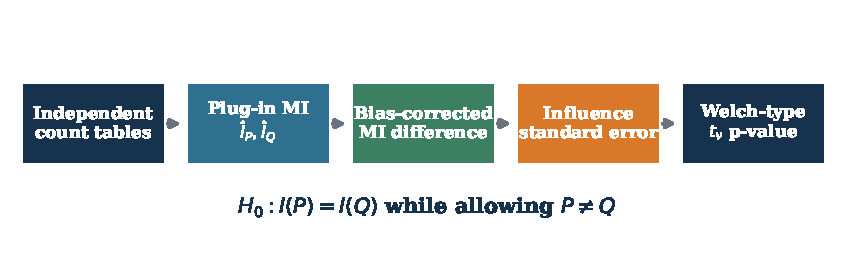
\includegraphics[width=0.96\textwidth]{method_overview.pdf}
  \caption{\textbf{Overview of \method.} Two independent contingency tables
  are converted to plug-in MI estimates, corrected for leading finite-sample
  bias, studentized with influence-function variances, and compared with a
  Welch-type Student reference. The target is equality of MI, not equality of
  the complete distributions and not independence within either table.}
  \label{fig:pipeline}
\end{figure*}

The contribution is a synthesis and evaluation rather than the invention of
its ingredients. Welch tests have previously been applied to collections of
MI estimates, and asymptotic comparisons of discrete MI values already exist.
The narrow contribution is, to our knowledge, the first systematic
finite-sample evaluation of this specific one-table-per-population
construction: bias-corrected discrete MI, empirical influence variance, and a
Welch--Satterthwaite reference under the unrestricted weak null
Eq.~\eqref{eq:null}.

\section{Related Work}

\subsection{Finite-sample estimation of mutual information}

For an \(r\times c\) discrete distribution \(P=(p_{ij})\), MI is
\begin{equation}
  \MI(P)=\sum_{i=1}^{r}\sum_{j=1}^{c}
  p_{ij}\log\frac{p_{ij}}{p_{i+}p_{+j}}.
  \label{eq:mi}
\end{equation}
Replacing probabilities by empirical proportions gives the maximum-likelihood
or plug-in estimator. Its simplicity hides a systematic finite-sample upward
bias. Miller's entropy correction \citep{miller1955}, subsequent MI-specific
calculations \citep{moddemeijer1989}, and broader analyses
\citep{paninski2003} show why sparse sampling can contaminate information
estimates even after a leading correction.

For fixed positive support, the plug-in MI estimator is asymptotically normal
away from independence. Its first-order variance is the variance of the local
log density ratio \citep{moddemeijer1989}. Influence-function methods provide
a general language for this expansion and for information-theoretic
functionals more broadly \citep{kandasamy2015}. These results motivate fast
Wald inference, but the first-order influence function degenerates at exact
independence, where the chi-squared rather than normal limit is relevant.

\subsection{Comparing mutual information values}

The idea of comparing MI across populations is not new. Mora and
Ruiz-Castillo derived asymptotic inference and pairwise comparisons for a
discrete MI segregation index and recommended bootstrap methods in smaller
samples \citep{mora2009}. Hart and Giszter combined jackknife uncertainties
when comparing histogram MI estimates in neuroscience
\citep{hart2010}. These works are close mathematical predecessors to the
present two-sample problem.

Other studies apply familiar mean tests to \emph{replicated} MI estimates.
Sarkar and Pandey used a Student test on MI values obtained from randomized or
shuffled astronomical data \citep{sarkar2020}. Prince et al.\ applied Welch
comparisons to per-neuron MI outcomes \citep{prince2021}. Martin et al.\ used
an unequal-variance Welch test on repeated, non-overlapping partition
estimates from a continuous KSG estimator \citep{holmes2019,martin2026}.
These studies establish that Welch testing has entered MI applications. They
do not, however, derive the two variance components from one discrete
multinomial table per population as done here. Mather et al.\ evaluated
Welch and MI leakage detectors side by side, but did not apply the Welch
reference to the MI estimator itself \citep{mather2013}.

\subsection{Permutation under a weak null}

Raw permutation is exact when observations are exchangeable under the strong
null \(P=Q\). Under Eq.~\eqref{eq:null}, \(P\) and \(Q\) may differ in every
respect other than MI, so group labels are generally not exchangeable.
Consequently, naively permuting labels can test the wrong null. General
permutation theory shows that studentization can recover asymptotic validity
for equality of parameters under weak assumptions while retaining finite
exactness when the complete distributions are equal \citep{chung2013}. We
therefore use a studentized table-label permutation as the resampling
benchmark, rather than raw permutation or a one-table independence shuffle.

\section{Daniel's Method}

\subsection{Data and estimand}

Let \(N^P=(N^P_{ij})\) and \(N^Q=(N^Q_{ij})\) be independent \(r\times c\)
count tables with totals \(n_P\) and \(n_Q\). Categories must be aligned
between groups. Write \(\widehat p_{ij}=N^P_{ij}/n_P\) and define
\(\widehat q_{ij}\) analogously. All formulas use natural logarithms and
therefore report nats. Changing to bits multiplies the estimated difference
and its standard error by the same constant, leaving the test statistic and
p-value unchanged.

The parameter of interest is the signed differential MI
\begin{equation}
  \Delta=\MI(P)-\MI(Q).
\end{equation}
The test is two-sided by default, although a directional alternative follows
immediately when it is scientifically pre-specified.

\subsection{Bias-corrected effect estimate}

Let \(d=(r-1)(c-1)\). Under fixed positive support, the leading plug-in MI
bias is \(d/(2n)\). We therefore define
\begin{align}
  \widetilde{\MI}_P
    &= \widehat{\MI}_P-\frac{d}{2n_P},\\
  \widetilde{\MI}_Q
    &= \widehat{\MI}_Q-\frac{d}{2n_Q},\\
  \widehat\Delta_{\mathrm{BC}}
    &=\widetilde{\MI}_P-\widetilde{\MI}_Q.
  \label{eq:delta}
\end{align}
This correction is especially important when \(n_P\ne n_Q\), because the
uncorrected difference has leading bias
\(d(1/n_P-1/n_Q)/2\) even under equal population MI.

The correction uses the declared alphabet dimensions, not the observed
nonempty dimensions. It is appropriate for the stated fixed-positive-support
asymptotics. In a severely sparse sample it can overcorrect, and corrected MI
values may be negative. Neither clipping nor data-dependent support changes
are applied because both would alter the estimand and sampling expansion.

\subsection{Influence-function uncertainty}

For each positive cell, define local information
\begin{equation}
  \ell^P_{ij}=\log
  \frac{\widehat p_{ij}}{\widehat p_{i+}\widehat p_{+j}}.
\end{equation}
The empirical influence variance is
\begin{equation}
  \widehat V_P
  =\sum_{ij:\widehat p_{ij}>0}\widehat p_{ij}
   \left(\ell^P_{ij}-\widehat{\MI}_P\right)^2,
  \label{eq:variance}
\end{equation}
with \(\widehat V_Q\) defined analogously. Independence of the samples gives
\begin{equation}
  \widehat{\mathrm{SE}}
  =\sqrt{\frac{\widehat V_P}{n_P}
               +\frac{\widehat V_Q}{n_Q}}.
  \label{eq:se}
\end{equation}
The standardized statistic is
\begin{equation}
  T=\frac{\widehat\Delta_{\mathrm{BC}}}
          {\widehat{\mathrm{SE}}}.
  \label{eq:tstat}
\end{equation}
Equations~\eqref{eq:delta}--\eqref{eq:tstat} are identical to the
bias-corrected normal Wald baseline.

\subsection{Welch--Satterthwaite reference}

Set
\begin{equation}
  a=\frac{\widehat V_P}{n_P},
  \qquad
  b=\frac{\widehat V_Q}{n_Q}.
\end{equation}
\method{} assigns the effective degrees of freedom
\begin{equation}
  \widehat\nu
  =\frac{(a+b)^2}
  {a^2/(n_P-1)+b^2/(n_Q-1)}.
  \label{eq:df}
\end{equation}
The two-sided p-value and \(100(1-\alpha)\%\) confidence interval are
\begin{align}
  p_{\mathrm{D}}
    &=2\Pr\{t_{\widehat\nu}\ge |T|\},\\
  \widehat\Delta_{\mathrm{BC}}
    &\ \pm\
    t_{\widehat\nu,1-\alpha/2}\widehat{\mathrm{SE}}.
  \label{eq:pvalue}
\end{align}
For finite \(\widehat\nu\), Student tails are heavier than normal tails.
Thus, at a fixed \(T\), \(p_{\mathrm{D}}\) is never smaller than the normal
Wald p-value. The method is a transparent conservative adjustment, not a new
effect estimator.

\begin{table}[t]
\centering
\caption{\textbf{Operational algorithm for one comparison.}}
\label{tab:algorithm}
\begin{tabular}{@{}p{0.06\columnwidth}p{0.86\columnwidth}@{}}
\toprule
1 & Validate two aligned, independent count tables.\\
2 & Compute plug-in MI in each table using Eq.~\eqref{eq:mi}.\\
3 & Subtract \(d/(2n)\) and form the difference in Eq.~\eqref{eq:delta}.\\
4 & Compute local-information variances using Eq.~\eqref{eq:variance}.\\
5 & Form the standard error and statistic in Eqs.~\eqref{eq:se}--\eqref{eq:tstat}.\\
6 & Compute \(\widehat\nu\) from Eq.~\eqref{eq:df}.\\
7 & Return the Student p-value, confidence interval, and support diagnostics.\\
\bottomrule
\end{tabular}
\end{table}

\subsection{First-order justification and qualification}

For a positive fixed table,
\begin{equation}
  \sqrt{n}\{\widehat{\MI}-\MI(P)\}
  =
  \frac{1}{\sqrt{n}}\sum_{k=1}^{n}
  \psi_P(X_k,Y_k)+o_P(1),
  \label{eq:linear}
\end{equation}
where
\(\psi_P(x,y)=\log\{p_{xy}/(p_{x+}p_{+y})\}-\MI(P)\)
is the MI influence function. Combining the independent
expansions for \(P\) and \(Q\) establishes the normal-reference Wald limit.

\begin{proposition}
Assume fixed finite alphabets, positive population cell probabilities,
independent and identically distributed observations within each group,
independent groups, \(n_P/(n_P+n_Q)\to\lambda\in(0,1)\), and positive
influence variances. Under \(H_0\), the statistic \(T\) in
Eq.~\eqref{eq:tstat} converges in distribution to \(N(0,1)\).
Furthermore, \(\widehat\nu\to\infty\), so the Student reference in
Eq.~\eqref{eq:pvalue} converges to the same normal limit.
\end{proposition}

The proposition establishes first-order compatibility, not exact
finite-sample validity. Classical Welch inference combines ordinary sample
variances with known Gaussian degrees-of-freedom interpretations. Here,
\(\widehat V_P\) and \(\widehat V_Q\) are nonlinear plug-in functionals:
the local scores change with the same empirical tables used to estimate MI.
Assigning \(n_P-1\) and \(n_Q-1\) in Eq.~\eqref{eq:df} is therefore a
Welch--Satterthwaite \emph{analogy}. Its value must be evaluated empirically.

\subsection{Worked numerical example}

Consider the following synthetic \(3\times3\) tables:
\begin{equation*}
N^P=
\begin{pmatrix}
45&15&10\\
15&45&10\\
10&10&40
\end{pmatrix},
\qquad
N^Q=
\begin{pmatrix}
48&32&20\\
32&48&20\\
20&20&40
\end{pmatrix}.
\end{equation*}
Their totals are \(n_P=200\) and \(n_Q=280\), and \(d=4\). The plug-in
estimates are 0.211316 and 0.054303 nats. Subtracting 0.010000 and 0.007143
gives corrected estimates 0.201316 and 0.047160, hence
\(\widehat\Delta_{\mathrm{BC}}=0.154155\) nats.

The empirical influence variances are \(\widehat V_P=0.395412\) and
\(\widehat V_Q=0.110863\). Therefore,
\[
  \widehat{\mathrm{SE}}
  =\sqrt{0.395412/200+0.110863/280}
  =0.048713,
\]
and \(T=3.16454\). Equation~\eqref{eq:df} gives
\(\widehat\nu=278.71\). The normal p-value is 0.001553, whereas \method{}
returns \(p=0.001725\) and a 95\% interval
\([0.05826,0.25005]\) nats. Both references reject equality, but the Student
reference is slightly more conservative. The minimum independence-expected
counts are 18.0 and 22.9, so this example lies comfortably inside the dense
regular regime. It illustrates the calculation only and is not part of the
simulation evidence.

\subsection{Complexity and recommended output}

Given two count tables, plug-in MI, influence variance, and support
diagnostics each require a constant number of scans over \(rc\) cells.
Consequently, time is \(O(rc)\) and additional working memory is \(O(rc)\)
in the vectorized implementation. If raw observation pairs are supplied,
forming the tables first adds \(O(n_P+n_Q)\) time. No random number generator,
resample count, or convergence tolerance is required.

A complete analysis should report \(n_P,n_Q,r,c\), the two plug-in and
bias-corrected MI estimates, \(\widehat\Delta_{\mathrm{BC}}\),
\(\widehat{\mathrm{SE}}\), \(T\), \(\widehat\nu\), the Student p-value and
confidence interval, and the normal-reference p-value as a comparator.
Zero-cell fractions and expected-count diagnostics should accompany sparse
applications. A noncomputable first-order variance must be reported as
invalid, not silently converted to \(p=1\). The bias correction and the
Welch reference are distinct: the former changes the point estimate, while
the latter changes only the inferential reference.

\section{Experimental Design}

\subsection{Weak-null population construction}

Every null experiment used independent multinomial samples from population
pairs satisfying \(\MI(P)=\MI(Q)\) to numerical tolerance while allowing
different margins and joint distributions. Random Dirichlet margins and
interaction structures generated heterogeneous tables, and association
strength was adjusted to target MI levels of 0.03, 0.07, or 0.15 nats. Common
sampled table pairs were supplied to all methods, producing paired method
comparisons without training, threshold fitting, or cross-method data
leakage.

\subsection{Decisive simulation}

The main experiment contained four stages:
\begin{enumerate}[leftmargin=1.3em,itemsep=1pt,topsep=2pt]
  \item A broad grid of 144 population pairs, shapes from \(2\times2\) to
  \(20\times20\), square and rectangular tables, equal and unequal samples
  with ratios 1:1, 1:2, and 1:4, and 5,000 replicates per pair.
  \item A targeted hard grid of 12 low-density, unequal-sample population
  pairs across six shapes, with 20,000 fresh replicates per pair.
  \item A 26-scenario stress grid with sample sizes 20--200 and 10,000
  replicates per scenario. This deliberately approached or crossed the
  first-order boundary.
  \item Five \(3\times3\) power scenarios with true differences 0.02, 0.05,
  and 0.10 nats and 10,000 replicates each.
\end{enumerate}
In total, the decisive run evaluated 1,220,000 null table pairs and 50,000
power pairs. Twelve thousand hard-grid pairs also received 999 optimized
studentized table permutations.

\subsection{Independent adversarial holdout}

After the decisive results were inspected, a separate audit fixed new
population, simulation, and bootstrap seeds. It generated 72 fresh weak-null
population pairs with 10,000 table pairs each, re-evaluated six frozen hard
designs with 10,000 fresh table pairs each, and generated 72 strong-null
\(P=Q\) scenarios with 5,000 table pairs each. This holdout added 1.14 million
table-pair evaluations and was designed to test the direction and
generalizability of the observed effect rather than tune the method.

\subsection{Comparators and metrics}

The primary analytic comparator was the bias-corrected normal Wald test,
which shares the estimate, standard error, and statistic with \method. The
resampling comparator was a studentized analytic table-label permutation
test. An exploratory variant using \(n-1\) rather than \(n\) in the empirical
variance denominator was reported separately but was not used to define the
primary method.

At nominal \(\alpha=0.05\) and 0.10, we recorded false-positive rate (FPR),
Wilson intervals, mean absolute FPR error (MAE), confidence-interval coverage,
valid-result rate, paired rejection changes, power, and runtime. Calibration
is the central criterion: at \(\alpha=0.05\), an ideal method has FPR 0.05,
and smaller \(|\mathrm{FPR}-0.05|\) is better.

\section{Results}

\subsection{Calibration}

Table~\ref{tab:calibration} summarizes the decisive null experiment. In the
broad regular grid, both analytic methods were well calibrated: mean FPR was
0.04977 for normal Wald and 0.04951 for \method. MAE improved slightly from
0.00514 to 0.00504, and the proportion of scenarios within the practical
0.035--0.065 band increased from 97.22\% to 97.92\%.

\begin{table*}[t]
\centering
\caption{\textbf{Decisive null calibration at nominal \(\alpha=0.05\).}
The stress grid is outside or near the intended first-order operating
boundary. MAE is mean absolute false-positive-rate error.}
\label{tab:calibration}
\small
\begin{tabular}{@{}llrrrrr@{}}
\toprule
Grid & Method & Scenarios & Mean FPR & MAE & 95\% coverage & In 3.5--6.5\% band\\
\midrule
Broad & Normal Wald & 144 & 0.04977 & 0.00514 & 0.95023 & 97.22\%\\
Broad & \method & 144 & 0.04951 & 0.00504 & 0.95049 & 97.92\%\\
\addlinespace
Hard & Normal Wald & 12 & 0.06177 & 0.01177 & 0.93823 & 75.00\%\\
Hard & \method & 12 & 0.06084 & 0.01084 & 0.93916 & 91.67\%\\
\addlinespace
Stress & Normal Wald & 26 & 0.06580 & 0.03180 & 0.93420 & 19.23\%\\
Stress & \method & 26 & 0.06276 & 0.03037 & 0.93724 & 15.38\%\\
\bottomrule
\end{tabular}
\end{table*}

The targeted hard grid was deliberately liberal under normal Wald. Its mean
FPR fell from 0.06177 to 0.06084, and MAE fell from 0.01177 to 0.01084, a
7.9\% relative reduction. Welch removed 224 normal-Wald rejections among
240,000 hard-null pairs; no Welch-only rejection is possible because the
Student p-value is nested above the normal p-value. Coverage increased by
0.00093.

The stress grid shows the limit of the reference correction. Mean FPR moved
toward 0.05, but scenario-level behaviour was not uniformly better. Already
conservative \(2\times2\) settings became more conservative, and 34
first-order-degenerate cases were explicitly returned as invalid. The 99.987\%
valid rate is high, but stress-grid FPR is conditional on a computable
positive standard error.

\begin{figure*}[t]
  \centering
  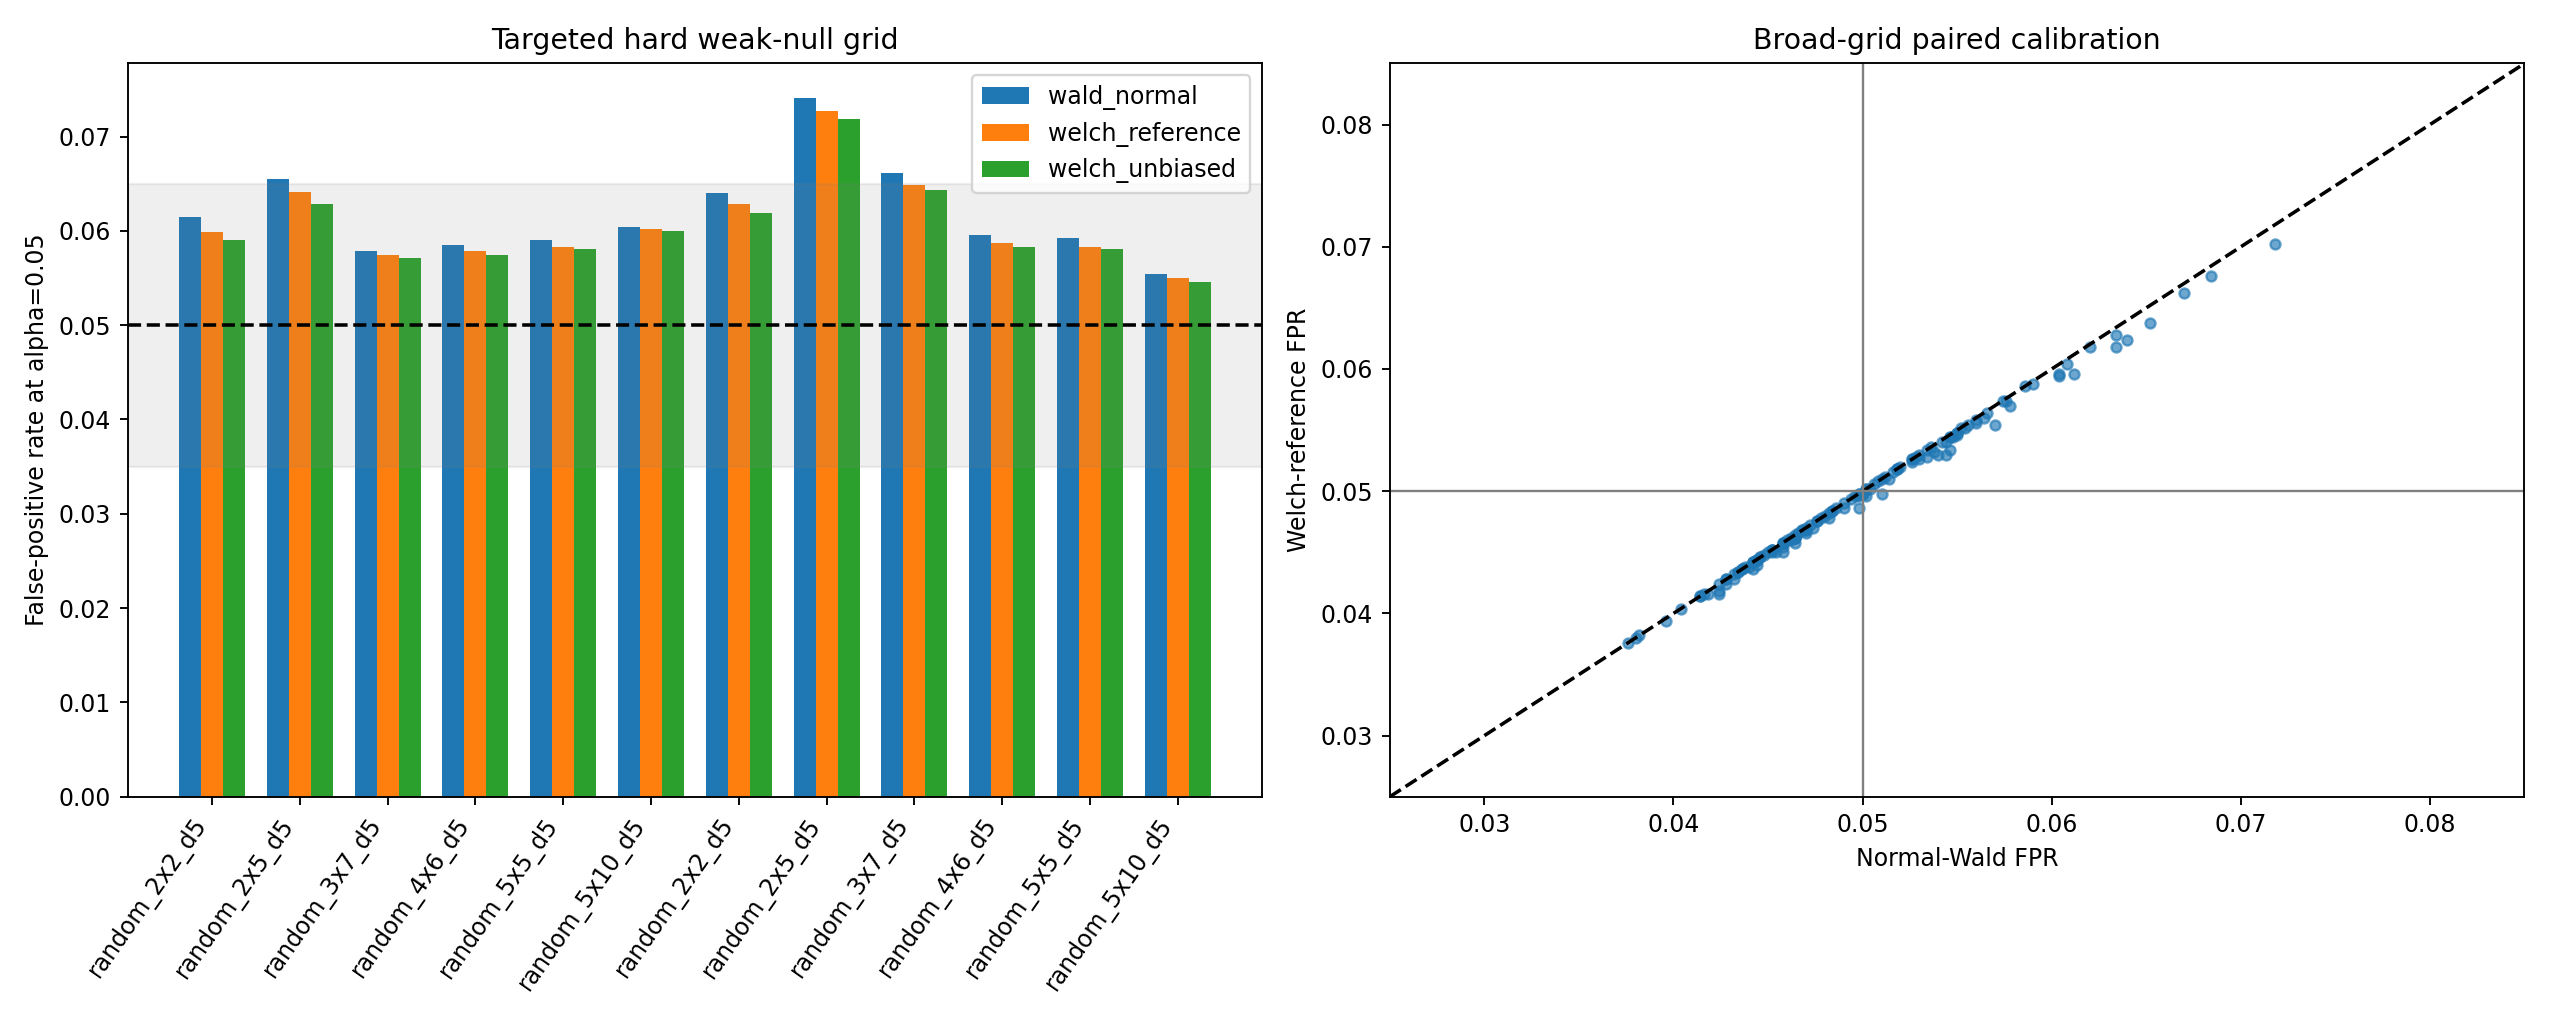
\includegraphics[width=\textwidth]{calibration_comparison.png}
  \caption{\textbf{Paired calibration in the decisive simulation.}
  Left: hard-grid FPRs for the normal baseline, primary Welch reference, and
  exploratory unbiased-variance sensitivity. The dashed line is nominal
  0.05 and the shaded band is 0.035--0.065. Right: each point is one broad
  scenario; points below the diagonal indicate a lower rejection rate under
  \method. The adjustment is intentionally small because hard-grid median
  effective degrees of freedom ranged from approximately 186 to 812.}
  \label{fig:calibration}
\end{figure*}

\subsection{Independent holdout}

The holdout reproduced the direction of the effect without reusing the broad
population pairs (Table~\ref{tab:holdout}). In the fresh weak-null broad
grid, mean MAE gain was 0.000210 with a scenario-bootstrap 95\% interval
[0.000090, 0.000344]. In all six frozen hard designs, \method{} improved
calibration; mean gain was 0.001283 [0.000917, 0.001650]. The fresh strong-null
grid also showed a small positive average gain. These results support a real
conservative effect, but not uniform superiority: in the fresh broad grid,
26 scenarios improved, 14 worsened, and 32 tied.

\begin{table*}[t]
\centering
\caption{\textbf{Adversarial holdout at nominal \(\alpha=0.05\).}
Intervals are scenario-bootstrap intervals for the mean MAE gain
\((\mathrm{MAE}_{N}-\mathrm{MAE}_{D})\).}
\label{tab:holdout}
\small
\begin{tabular}{@{}lrrrrr@{}}
\toprule
Holdout stage & Population pairs & Tables per pair & Normal MAE & Daniel MAE &
Mean gain [95\% interval]\\
\midrule
Fresh weak-null broad & 72 & 10,000 & 0.004792 & 0.004582 &
0.000210 [0.000090, 0.000344]\\
Frozen hard design & 6 & 10,000 & 0.009083 & 0.007800 &
0.001283 [0.000917, 0.001650]\\
Fresh strong null & 72 & 5,000 & 0.005142 & 0.004958 &
0.000183 [0.000064, 0.000322]\\
\bottomrule
\end{tabular}
\end{table*}

\subsection{Permutation comparison}

Studentized permutation remained the most accurate comparator in the hard
anchors (Table~\ref{tab:permutation}). Its mean FPR was 0.05458 and MAE was
0.00642, versus 0.06083 and 0.01100 for \method{} on the same 12 anchor
sets. Every permutation anchor was inside the practical calibration band.
Thus, \method{} closes only part of the gap between normal analytic inference
and resampling; it does not replace permutation when maximum finite-sample
calibration is worth the additional computation.

\begin{table}[t]
\centering
\caption{\textbf{Hard-grid permutation anchors.} Each of 12 scenarios used
1,000 table pairs and 999 studentized permutations.}
\label{tab:permutation}
\small
\setlength{\tabcolsep}{3pt}
\begin{tabular}{@{}lrrr@{}}
\toprule
Method & Mean FPR & MAE & In band\\
\midrule
Normal Wald & 0.06208 & 0.01208 & 66.67\%\\
\method & 0.06083 & 0.01100 & 75.00\%\\
Studentized permutation & 0.05458 & 0.00642 & 100.00\%\\
\bottomrule
\end{tabular}
\end{table}

\subsection{Power and computation}

The heavier Student tail produces a predictable but small power cost.
Across five power scenarios, mean absolute loss relative to normal Wald was
0.00154; the largest scenario-level loss was 0.0032 at \(n_P=n_Q=150\).
For a 0.05-nat effect at \(n=300\), power changed from 0.2776 to 0.2761.
For a 0.10-nat effect, it changed from 0.7438 to 0.7419.

Median single-pair runtime was 0.117 ms for normal Wald and 0.128 ms for
\method, a 9.1\% relative overhead but only 0.011 ms in absolute terms.
Across the 12 permutation anchors, median time for 999 permutations was
3.006 ms, with a range from roughly 1.1 to 5.9 ms depending on table shape.
The implementation is vectorized, so the exact ratio depends on batching and
hardware. The key distinction is algorithmic: the analytic calculation scans
the \(rc\) cells once, whereas permutation repeats table allocation and
studentized MI evaluation \(B\) times.

\begin{figure*}[t]
  \centering
  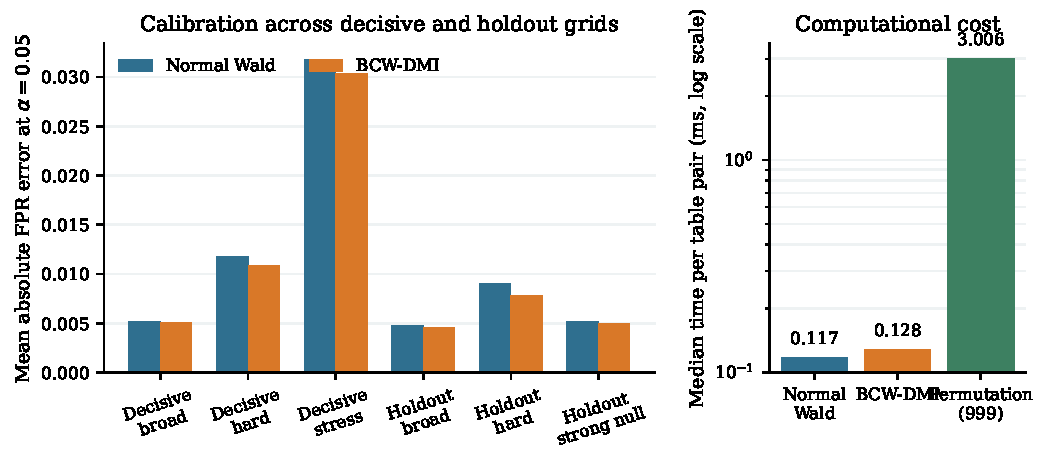
\includegraphics[width=\textwidth]{evidence_summary.pdf}
  \caption{\textbf{Accuracy and cost summary.} Left: normal and Daniel MAE
  across the decisive study and independent holdout. The largest benefit
  occurs in deliberately liberal hard regimes; broad and strong-null effects
  are small. Right: median observed single-pair runtime on a logarithmic
  scale. The permutation result uses 999 optimized table permutations and is
  not JIDT's one-table independence shuffle.}
  \label{fig:evidence}
\end{figure*}

\section{Adversarial Audit}

\subsection{Correctness and reproducibility}

The implementation passed direct hand calculations of MI, bias, variance,
degrees of freedom, statistic, and p-value. Swapping groups and relabelling
rows or columns left the p-value unchanged. Student p-values were never
smaller than their normal counterparts, and the two references converged at
large sample size. Natural-log units were used consistently. All valid
p-values were finite and inside \([0,1]\); malformed tables and degenerate
first-order variances were rejected explicitly.

Simulation streams were separated across population generation, table
sampling, permutation, and power experiments. The weak null held to a maximum
saved numerical discrepancy of \(9.3\times10^{-14}\) nats. Reconstructing
saved replicates from scenario and simulation seeds reproduced estimates and
p-values to floating-point precision. No fitted hyperparameter, learned
threshold, or training stage consumed validation outcomes.

\subsection{Degrees-of-freedom limitation}

The central theoretical qualification is visible in
Fig.~\ref{fig:dfaudit}. In five representative populations, the implemented
naive total degrees of freedom ranged from 171 to 858, whereas empirical
moment-matched values ranged from 28 to 196. A separately derived influence
function for the variance functional predicted 26 to 181 and tracked the
empirical values more closely.

\begin{figure}[t]
  \centering
  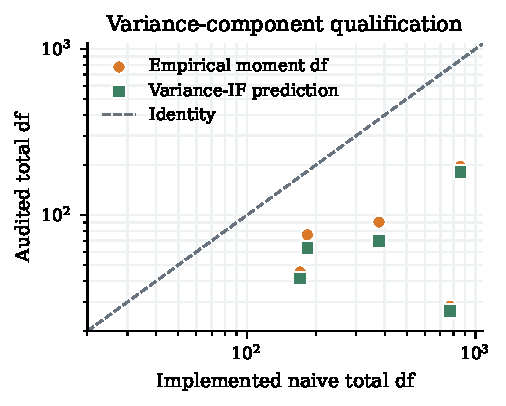
\includegraphics[width=\columnwidth]{df_audit.pdf}
  \caption{\textbf{The implemented degrees of freedom are heuristic.}
  Empirical moment degrees of freedom for the total estimated variance are
  well below Eq.~\eqref{eq:df}. A variance-functional influence calculation
  tracks the audit more closely. The current procedure must therefore be
  described as Welch-inspired, not exact.}
  \label{fig:dfaudit}
\end{figure}

This discrepancy does not invalidate the first-order asymptotic result:
every candidate reference converges to normal as sample size grows. It does
show that Eq.~\eqref{eq:df} is not literally moment matching the sampling
distribution of the nonlinear influence-variance estimator. Correlation
between the estimated MI difference and its total estimated variance reached
0.84 in a skewed \(2\times2\) audit, so improving the denominator degrees of
freedom alone may still not yield an exact Student law.

\subsection{Post-protocol decision}

The frozen validation protocol used an internal rule requiring at least a
20\% reduction in hard-grid MAE. The observed 7.9\% reduction did not satisfy
that rule, and the generated metadata correctly records ``NO-GO.'' The later
decision to retain the method as a thesis contribution accepts a smaller
effect as scientifically useful. This is a transparent post-protocol change
in materiality judgement, not a pre-specified success. The numerical result,
comparators, and frozen report were not altered.

\section{Discussion}

\subsection{What the method adds}

\method{} occupies a practical middle ground. Relative to normal analytic
inference, it adds almost no computational burden, preserves large-sample
behaviour, and provides a small conservative adjustment where the baseline
is mildly liberal. Relative to studentized permutation, it is less accurately
calibrated but deterministic and faster. It is most attractive in screening
or repeated-comparison settings where milliseconds accumulate, exact
reproducibility is valuable, and a modest calibration improvement is useful.

The size of the improvement is mathematically unsurprising. In the hard grid,
median effective degrees of freedom were approximately 186--812. Student
critical values at those degrees of freedom are close to normal critical
values, so few decisions change. This modest effect is a feature of a
backward-compatible reference correction: the estimate and uncertainty model
remain untouched.

\subsection{Relationship to standard MI tests}

Table~\ref{tab:methods} separates four procedures that are easily conflated.
Chi-squared and JIDT shuffling address independence within one population.
They are appropriate for \(H_0:\MI(P)=0\), not Eq.~\eqref{eq:null}. Normal
Wald, \method, and studentized two-sample permutation address equal MI across
independent populations. Raw group-label permutation is exact only under the
stronger \(P=Q\) null; studentization is required for the heterogeneous weak
null.

\begin{table*}[t]
\centering
\caption{\textbf{How the proposed procedure relates to common significance
methods.} A method is only a valid comparator when it targets the same null.}
\label{tab:methods}
\small
\begin{tabular}{@{}p{0.19\textwidth}p{0.22\textwidth}p{0.18\textwidth}p{0.31\textwidth}@{}}
\toprule
Method & Null hypothesis & Computation & Role\\
\midrule
Chi-squared / JIDT analytic & \(\MI(P)=0\) & Closed-form reference &
One-table independence; not a test of equal MI across groups.\\
JIDT variable shuffling & \(\MI(P)=0\) & Repeated data-label shuffles &
One-table empirical independence significance; not a direct comparator.\\
Bias-corrected normal Wald & \(\MI(P)=\MI(Q)\) & \(O(rc)\), deterministic &
Historical two-sample analytic baseline.\\
\method & \(\MI(P)=\MI(Q)\) & \(O(rc)\), deterministic &
Proposed mildly conservative finite-df refinement.\\
Studentized group permutation & \(\MI(P)=\MI(Q)\) asymptotically; exact if \(P=Q\) &
\(B\) repeated allocations and evaluations &
More accurate regular resampling benchmark, with higher cost.\\
\bottomrule
\end{tabular}
\end{table*}

\subsection{Novelty boundary}

No broad claim that Welch has never been used with MI is sustainable.
Published examples use Welch on repeated continuous-MI estimates
\citep{martin2026}, per-unit MI outcomes \citep{prince2021}, and related
information measures. Nor are the plugin estimator, \(d/(2n)\) correction,
influence variance, two-sample studentization, or Satterthwaite formula
individually new.

The defensible contribution is narrower: a complete, deterministic,
MI-specific procedure for two independent discrete tables under the weak
equal-MI null, together with unusually broad finite-sample calibration,
permutation comparison, reproducibility checks, and an adversarial audit of
the degrees-of-freedom assumption. A structured search did not locate the
same combination. Before any publication-priority statement, the search
should be repeated in authenticated Scopus, Web of Science, MathSciNet,
zbMATH, and ProQuest databases.

\subsection{Limitations and operating range}

The method requires independent observations within each group and independent
groups; fixed, aligned categorical alphabets; positive population support;
sample-size proportions bounded away from zero and one; and nonzero
population influence variance. It does not currently cover paired,
clustered, longitudinal, or time-series samples.

Exact and near independence are outside scope because the first-order MI
influence function degenerates. Structural zeros, unknown support, severe
sampling sparsity, or alphabets growing with sample size can invalidate both
the leading bias correction and variance approximation. The reported
zero-cell and expected-count diagnostics describe a table but are not proven
validity rules. Conditional MI, transfer entropy, and continuous MI require
new derivations.

The simulation evidence is extensive in null calibration but less broad in
power: the five alternatives are \(3\times3\) tables with equal sample sizes.
The permutation comparison covers 12 hard anchors with 1,000 outer replicates
each. A final thesis study should broaden power across shapes and unequal
samples, increase the outer permutation replicates, include
\(\alpha=0.01\), and add real-data demonstrations. These additions improve
external validity; simply increasing the existing null replicate counts would
add little.

\subsection{Next methodological step}

The variance-functional audit suggests a principled extension. If
\(\tau_P^2\) denotes the variance of the influence function of
\(\widehat V_P\), first-order moment matching gives a component degree of
freedom of approximately \(2n_PV(P)^2/\tau_P^2\), with an analogous term for
\(Q\). This prediction tracked empirical component degrees of freedom more
closely than \(n-1\). It must be frozen and tested on untouched populations
before replacing Eq.~\eqref{eq:df}. Corrected Satterthwaite formulas proposed
for general variance synthesis may also be relevant \citep{vondavier2026},
but their assumptions are not yet established for MI.

\section{Conclusion}

\method{} adapts a familiar statistical idea to a distinct information-
theoretic problem: fast inference for equality of two independent discrete
mutual information values. It combines leading plug-in bias correction,
influence-function uncertainty, and a Welch--Satterthwaite-inspired reference
without resampling. Across a large pre-specified simulation and an independent
holdout, it produced a small, reproducible conservative calibration
improvement over normal Wald with negligible power and runtime costs.
Studentized permutation remained more accurate.

The result should be interpreted precisely. This is not an exact Welch theorem
for MI, not a one-table independence test, and not a solution to severe
sparsity. Its value is a clean and general regular-case refinement, an
auditable implementation, and a quantitative map of where the approximation
helps and where first-order MI inference remains inadequate.

\section*{Reproducibility and Data Availability}

The implementation, frozen protocol, experiment runners, aggregate result
tables, seeds, environment metadata, tests, and figure-generation code are
stored in the accompanying research repository. The full null replicate
archive is reproducible from the saved scenario definitions and seeds but is
not versioned because of its size. The manuscript figures are generated by
\texttt{article/make\_figures.py}; the decisive experiment is generated by
\texttt{experiments/run\_validation.py}. The method implementation is
\texttt{src/welch\_differential\_mi/welch.py}.

\section*{Acknowledgements}

This draft was prepared as part of a master's research project. Formal
supervisor, institutional, funding, conflict-of-interest, and author-
contribution statements should be inserted before submission.

\bibliographystyle{unsrtnat}
\bibliography{references}

\end{document}
